% Stat 696: Knitr illustration for online video
% Illustrating knitr to present analyses of College data from ISLR text
% Packages required: knitr, xtable, stargazer, ISLR
% To use, make sure to call library(knitr) first in console
% To run and create a .tex file: knit('knitr_ClassVersion.Rnw') in R
% August 24, 2017

% Preface required in the knitr RnW file
\documentclass{article}\usepackage[]{graphicx}\usepackage[]{color}
% maxwidth is the original width if it is less than linewidth
% otherwise use linewidth (to make sure the graphics do not exceed the margin)
\makeatletter
\def\maxwidth{ %
  \ifdim\Gin@nat@width>\linewidth
    \linewidth
  \else
    \Gin@nat@width
  \fi
}
\makeatother

\definecolor{fgcolor}{rgb}{0.345, 0.345, 0.345}
\newcommand{\hlnum}[1]{\textcolor[rgb]{0.686,0.059,0.569}{#1}}%
\newcommand{\hlstr}[1]{\textcolor[rgb]{0.192,0.494,0.8}{#1}}%
\newcommand{\hlcom}[1]{\textcolor[rgb]{0.678,0.584,0.686}{\textit{#1}}}%
\newcommand{\hlopt}[1]{\textcolor[rgb]{0,0,0}{#1}}%
\newcommand{\hlstd}[1]{\textcolor[rgb]{0.345,0.345,0.345}{#1}}%
\newcommand{\hlkwa}[1]{\textcolor[rgb]{0.161,0.373,0.58}{\textbf{#1}}}%
\newcommand{\hlkwb}[1]{\textcolor[rgb]{0.69,0.353,0.396}{#1}}%
\newcommand{\hlkwc}[1]{\textcolor[rgb]{0.333,0.667,0.333}{#1}}%
\newcommand{\hlkwd}[1]{\textcolor[rgb]{0.737,0.353,0.396}{\textbf{#1}}}%
\let\hlipl\hlkwb

\usepackage{framed}
\makeatletter
\newenvironment{kframe}{%
 \def\at@end@of@kframe{}%
 \ifinner\ifhmode%
  \def\at@end@of@kframe{\end{minipage}}%
  \begin{minipage}{\columnwidth}%
 \fi\fi%
 \def\FrameCommand##1{\hskip\@totalleftmargin \hskip-\fboxsep
 \colorbox{shadecolor}{##1}\hskip-\fboxsep
     % There is no \\@totalrightmargin, so:
     \hskip-\linewidth \hskip-\@totalleftmargin \hskip\columnwidth}%
 \MakeFramed {\advance\hsize-\width
   \@totalleftmargin\z@ \linewidth\hsize
   \@setminipage}}%
 {\par\unskip\endMakeFramed%
 \at@end@of@kframe}
\makeatother

\definecolor{shadecolor}{rgb}{.97, .97, .97}
\definecolor{messagecolor}{rgb}{0, 0, 0}
\definecolor{warningcolor}{rgb}{1, 0, 1}
\definecolor{errorcolor}{rgb}{1, 0, 0}
\newenvironment{knitrout}{}{} % an empty environment to be redefined in TeX

\usepackage{alltt}

\usepackage{rotating}
\usepackage{graphics}
\usepackage{latexsym}
\usepackage{color}
\usepackage{listings} % allows for importing code scripts into the tex file
\usepackage{wrapfig} % allows wrapping text around a figure
\usepackage{lipsum} % provides Latin text to fill up a page in this illustration (do not need it otherwise!)

% Approximately 1 inch borders all around
\setlength\topmargin{-.56in}
\setlength\evensidemargin{0in}
\setlength\oddsidemargin{0in}
\setlength\textwidth{6.49in}
\setlength\textheight{8.6in}

% Options for code listing; from Patrick DeJesus, October 2016
\definecolor{codegreen}{rgb}{0,0.6,0}
\definecolor{codegray}{rgb}{0.5,0.5,0.5}
\definecolor{codepurple}{rgb}{0.58,0,0.82}
\definecolor{backcolour}{rgb}{0.95,0.95,0.92}
\lstdefinestyle{mystyle}{
	backgroundcolor=\color{backcolour},   commentstyle=\color{codegreen},
	keywordstyle=\color{magenta},
	numberstyle=\tiny\color{codegray},
	stringstyle=\color{codepurple},
	basicstyle=\footnotesize,
	breakatwhitespace=false,         
	breaklines=true,                 
	captionpos=b,                    
	keepspaces=true,                 
	numbers=left,                    
	numbersep=5pt,                  
	showspaces=false,                
	showstringspaces=false,
	showtabs=false,                  
	tabsize=2
}
%"mystyle" code listing set
\lstset{style=mystyle}
%\lstset{inputpath=appendix/}


\title{Stat 696, Example Application of \texttt{knitr}} 
\author{Professor Levine}
\IfFileExists{upquote.sty}{\usepackage{upquote}}{}
\begin{document} 
\maketitle

% Code to start knitr


%%%%%%%%%%%%%%%%%%%%%%%%%%%%%%%%%%%%%%%%%%%%%%%%%%%%%%%%%%%%
% Code snippet to load in libraries and data  
% THIS IS HOW R-CODE IS READ INTO LaTeX DOC WITH knitr
% Environment:  
% <<...>>=  
% [Code here] 
% @
%%%%%%%%%%%%%%%%%%%%%%%%%%%%%%%%%%%%%%%%%%%%%%%%%%%%%%%%%%%%


First let's present an R-dump of the top of the College data set.  We emphasize that you would not include this in your data analysis report.  In this document, we just wish to illustrate how this is done in \texttt{knitr}.
% Short view of the data
\begin{knitrout}
\definecolor{shadecolor}{rgb}{0.969, 0.969, 0.969}\color{fgcolor}\begin{kframe}
\begin{alltt}
\hlkwd{head}\hlstd{(College)}
\end{alltt}
\begin{verbatim}
##                              Private Apps Accept Enroll Top10perc Top25perc
## Abilene Christian University     Yes 1660   1232    721        23        52
## Adelphi University               Yes 2186   1924    512        16        29
## Adrian College                   Yes 1428   1097    336        22        50
## Agnes Scott College              Yes  417    349    137        60        89
## Alaska Pacific University        Yes  193    146     55        16        44
## Albertson College                Yes  587    479    158        38        62
##                              F.Undergrad P.Undergrad Outstate Room.Board Books
## Abilene Christian University        2885         537     7440       3300   450
## Adelphi University                  2683        1227    12280       6450   750
## Adrian College                      1036          99    11250       3750   400
## Agnes Scott College                  510          63    12960       5450   450
## Alaska Pacific University            249         869     7560       4120   800
## Albertson College                    678          41    13500       3335   500
##                              Personal PhD Terminal S.F.Ratio perc.alumni Expend
## Abilene Christian University     2200  70       78      18.1          12   7041
## Adelphi University               1500  29       30      12.2          16  10527
## Adrian College                   1165  53       66      12.9          30   8735
## Agnes Scott College               875  92       97       7.7          37  19016
## Alaska Pacific University        1500  76       72      11.9           2  10922
## Albertson College                 675  67       73       9.4          11   9727
##                              Grad.Rate Elite
## Abilene Christian University        60    No
## Adelphi University                  56    No
## Adrian College                      54    No
## Agnes Scott College                 59   Yes
## Alaska Pacific University           15    No
## Albertson College                   55    No
\end{verbatim}
\end{kframe}
\end{knitrout}


We can also present results in the text using {\tt Sexpr}.  For example, in the College data set, there are 19 variables and the sample size is $n = $ 777.  Now let us replicate the \LaTeX\ document we created earlier in this video.

Let us start with an example from {\tt stargazer}.  I cut-and-pasted the \LaTeX\ code created by stargazer in R.  Recall we added a caption and label to reference the table.  Table~\ref{descrips} presents summary statistics for the College data set.  {\em Here you would then provide a brief description of the variables and any interesting findings about the statistics displayed.}
% We <<echo=FALSE>> to ask knitr not to present the R code in the output.
% We use results="asis" to force knitr to present the table code for compiling in LaTeX.

% Table created by stargazer v.5.2.2 by Marek Hlavac, Harvard University. E-mail: hlavac at fas.harvard.edu
% Date and time: Thu, Sep 03, 2020 - 2:26:18 PM
\begin{table}[!htbp] \centering 
  \caption{Summary statistics for the ISLR College data set.} 
  \label{descrips} 
\begin{tabular}{@{\extracolsep{5pt}}lccccccc} 
\\[-1.8ex]\hline 
\hline \\[-1.8ex] 
Statistic & \multicolumn{1}{c}{N} & \multicolumn{1}{c}{Mean} & \multicolumn{1}{c}{St. Dev.} & \multicolumn{1}{c}{Min} & \multicolumn{1}{c}{Pctl(25)} & \multicolumn{1}{c}{Pctl(75)} & \multicolumn{1}{c}{Max} \\ 
\hline \\[-1.8ex] 
Apps & 777 & 3,001.638 & 3,870.201 & 81 & 776 & 3,624 & 48,094 \\ 
Accept & 777 & 2,018.804 & 2,451.114 & 72 & 604 & 2,424 & 26,330 \\ 
Enroll & 777 & 779.973 & 929.176 & 35 & 242 & 902 & 6,392 \\ 
Top10perc & 777 & 27.559 & 17.640 & 1 & 15 & 35 & 96 \\ 
Top25perc & 777 & 55.797 & 19.805 & 9 & 41 & 69 & 100 \\ 
F.Undergrad & 777 & 3,699.907 & 4,850.421 & 139 & 992 & 4,005 & 31,643 \\ 
P.Undergrad & 777 & 855.299 & 1,522.432 & 1 & 95 & 967 & 21,836 \\ 
Outstate & 777 & 10,440.670 & 4,023.016 & 2,340 & 7,320 & 12,925 & 21,700 \\ 
Room.Board & 777 & 4,357.526 & 1,096.696 & 1,780 & 3,597 & 5,050 & 8,124 \\ 
Books & 777 & 549.381 & 165.105 & 96 & 470 & 600 & 2,340 \\ 
Personal & 777 & 1,340.642 & 677.071 & 250 & 850 & 1,700 & 6,800 \\ 
PhD & 777 & 72.660 & 16.328 & 8 & 62 & 85 & 103 \\ 
Terminal & 777 & 79.703 & 14.722 & 24 & 71 & 92 & 100 \\ 
S.F.Ratio & 777 & 14.090 & 3.958 & 2.500 & 11.500 & 16.500 & 39.800 \\ 
perc.alumni & 777 & 22.744 & 12.392 & 0 & 13 & 31 & 64 \\ 
Expend & 777 & 9,660.171 & 5,221.768 & 3,186 & 6,751 & 10,830 & 56,233 \\ 
Grad.Rate & 777 & 65.463 & 17.178 & 10 & 53 & 78 & 118 \\ 
\hline \\[-1.8ex] 
\end{tabular} 
\end{table} 


\newpage
Let us now present an example from {\tt xtable}.  I cut-and-pasted the \LaTeX\ code created by xtable in R.  Recall that we added a caption and label to the table.  Table~\ref{reginf} presents inferences for regressing the number of applications on six variables in the College data set.  We note that no model selection was run nor in-depth model diagnostics.  We merely chose six variables we thought my be important just to illustrate this regression inference table using xtable!
% Note that we use the print function to ensure the xtable LaTeX code is produced by knitr.
% latex table generated in R 3.6.2 by xtable 1.8-4 package
% Thu Sep 03 14:26:18 2020
\begin{table}[ht]
\centering
\begin{tabular}{|l|rrrr|}
  \hline
 & Estimate & Std. Error & t value & Pr($>$$|$t$|$) \\ 
  \hline
(Intercept) & -985.95 & 204.82 & -4.81 & 0.00 \\ 
  PrivateYes & -291.62 & 133.28 & -2.19 & 0.03 \\ 
  EliteYes & 1745.00 & 151.74 & 11.50 & 0.00 \\ 
  Accept & 1.43 & 0.02 & 70.60 & 0.00 \\ 
  Outstate & -0.01 & 0.02 & -0.84 & 0.40 \\ 
  Room.Board & 0.17 & 0.05 & 3.35 & 0.00 \\ 
  Grad.Rate & 8.63 & 2.95 & 2.93 & 0.00 \\ 
   \hline
\end{tabular}
\caption{Inferences from regressing number of applications on whether the college is private or public,
                  whether the college is elite or not, acceptance rate, out of state tuition, room and board, and 
                  graduation rate.} 
\label{reginf}
\end{table}


\newpage
Let us now present an example of wrapping a figure with text in \LaTeX.  Recall in the introduction to \LaTeX\ video and examples, we had \LaTeX\ decide where to put the figure.  If you want to try and save space by wrapping text around a figure, you would use the wrapfigure environment.
% Notice that construction a figure in knitr requires setting the figure environment in LaTeX and then
%  drawing the figure in R to send to LaTeX (so knitr R snippet within a LaTeX coded environment.)

% Syntax for wrapfigure: \begin{wrapfigure}[lineheight]{position}{width}
% Position could be R/r, l/L, i/I, o/O (right, left, inside edge, outside edge; uppercase version allows the figure to float, lowercase "exactly here".
\begin{wrapfigure}{R}{0.5\textwidth} % second parameter specifies percentage of text width image should cover
\centering
% Note that we do not need the includegraphics command, knitr does that for us.
%  But we do need to tell knitr any graphic specifications such as graphic width.
\begin{knitrout}
\definecolor{shadecolor}{rgb}{0.969, 0.969, 0.969}\color{fgcolor}
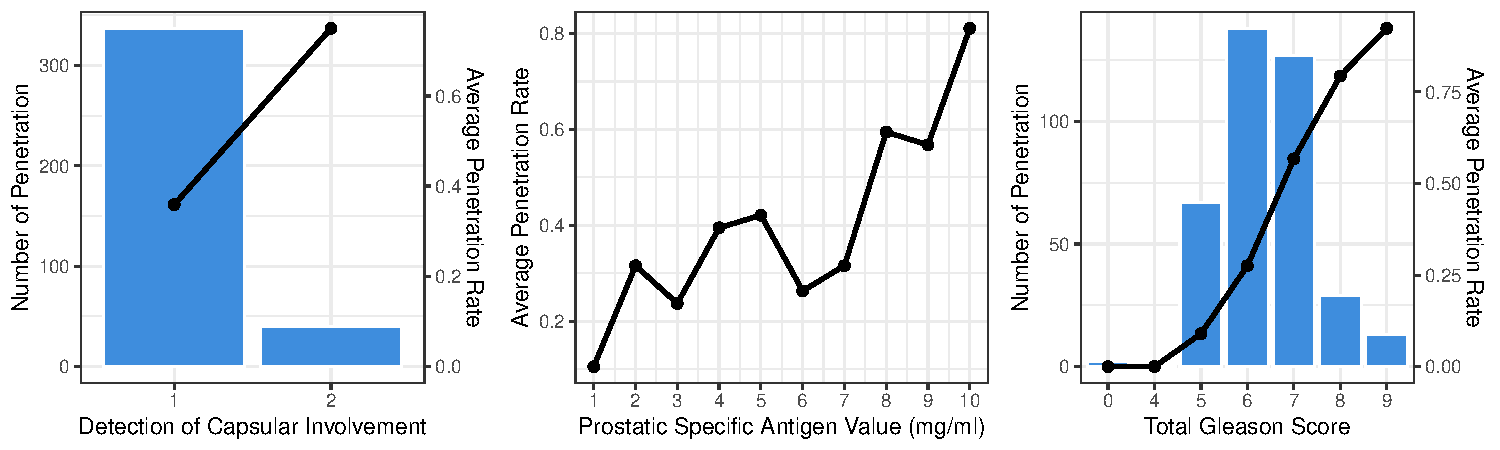
\includegraphics[width=0.45\textwidth]{figure/unnamed-chunk-2-1} 

\end{knitrout}
\caption{Box plot of out of state tuition against college elite status.}
\label{boxplot}
\end{wrapfigure}

\lipsum[1]
\lipsum[2]


% Create an appendix of code: we will present this knitr code here, not the Rtools.R code.
% The listing package in LaTeX provides a clean presentation of code in your report just by
% calling the R/Rnw file itself!
\newpage
\noindent \Large{{\bf R Code}}
\lstinputlisting[language=R, caption = Code Used for this knitr exercise]{knitr_ClassVersion.Rnw}
% All you need to change is the file name and caption.

\end{document}
